\section{Results}\label{sec:results}

\subsection{Execution-Time Model}

Across the 48 independent test transfers, 43 end-to-end durations fell below their grouped upper bounds, giving an aggregate empirical coverage of 89.6\%, close to the intended 90\% one-sided level (Table~\ref{tab:time-model}). Per-device coverage ranged from 83.3\% to 100.0\%. Mean upper margins were 5.917--6.823~s, while MAE ranged from 3.262 to 5.229~s and RMSE from 3.719 to 7.469~s. These errors are large relative to a purely mechanical short transfer because the response variable includes command handling, closed-loop arrival, stability, dwell, and the first qualifying post-arrival frame. The result supports using device- and direction-dependent end-to-end bounds in the planner; it does not establish an unconditional timing guarantee under network conditions outside the calibration runs.

The offline field-of-view sensitivity in Table~\ref{tab:core-sensitivity} shows a separate effect. A $1^\circ$ half-width retained a median 40.3\% of nominal cells per candidate and increased the planned task count from 5 to 16 relative to the uncontracted map. Its planned UAC and T100 were therefore higher than those at $0^\circ$ or $0.5^\circ$. The analysis clarifies the planning cost of the frozen feasible map. Because no hardware run was repeated under the alternative half-widths, the table cannot establish which half-width would yield the best physical performance.

\subsection{Nominal First-Coverage Performance}

All 70 hardware runs confirmed all 384 cells. Table~\ref{tab:nominal} summarizes the 30 nominal runs. Median UAC was 2.380~s for ECR-Cover, 7.480~s for MAG, and 3.070~s for the calibrated static route. The paired ECR-Cover-minus-MAG UAC median was $-4.941$~s with a 95\% bootstrap CI of $[-6.707,-3.910]$~s. All ten blocks favored ECR-Cover, giving a one-sided exact sign-test value of $p=0.0009766$. Relative to calibrated static planning, the paired median difference was $-0.265$~s with a 95\% CI of $[-1.046,-0.110]$~s. Figure~\ref{fig:nominal}a exposes the ten run-level observations through the empirical distributions, and Figure~\ref{fig:nominal}b reports the frozen paired intervals.

\begin{table*}[t]
\caption{Nominal hardware coverage, reported as median [IQR] over ten runs per method. Motion and load are deterministic plan-level summaries under the corresponding runs.}\label{tab:nominal}
\centering
\begin{tabular}{lccccc}
\toprule
Method & UAC (s) & T95 (s) & T100 (s) & Total angular motion (deg) & Load CV\\
\midrule
MAG & 7.480 [6.852, 8.173] & 18.152 [17.704, 19.653] & 18.152 [17.704, 19.653] & 304.264 & 0.143\\
Calibrated static & 3.070 [2.569, 3.330] & 12.653 [12.160, 12.903] & 20.340 [16.153, 24.399] & \textbf{290.140} & 0.474\\
\textbf{ECR-Cover} & \textbf{2.380 [2.286, 2.851]} & 12.837 [12.722, 12.895] & \textbf{12.891 [12.819, 14.800]} & 301.169 & 0.577\\
\bottomrule
\end{tabular}
\end{table*}

The T95 medians of ECR-Cover and calibrated static planning were similar, but their completion tails differed. ECR-Cover reduced median T100 by 6.066~s relative to the calibrated static method, with a paired 95\% CI of $[-10.620,-1.916]$~s. For ECR-Cover versus MAG, the paired T100 ratio had a median of 0.723 and a 95\% CI of $[0.647,0.807]$, below the 1.05 noninferiority threshold. Figure~\ref{fig:nominal}c shows that the ECR-Cover completion observations were concentrated below both comparison tails. The UAC reduction was therefore not obtained by postponing the last cells.

Total angular motion did not show a resolved difference from MAG because its paired-difference interval crossed zero. ECR-Cover had a larger load CV than MAG. This outcome follows the declared objective hierarchy: early viewpoints with a large marginal cell contribution can be assigned to the cameras that realize them earliest, even if that makes task counts less balanced. Load balance is a tie-break quantity rather than an objective allowed to displace UAC or T100.

\begin{figure*}[t]
\centering
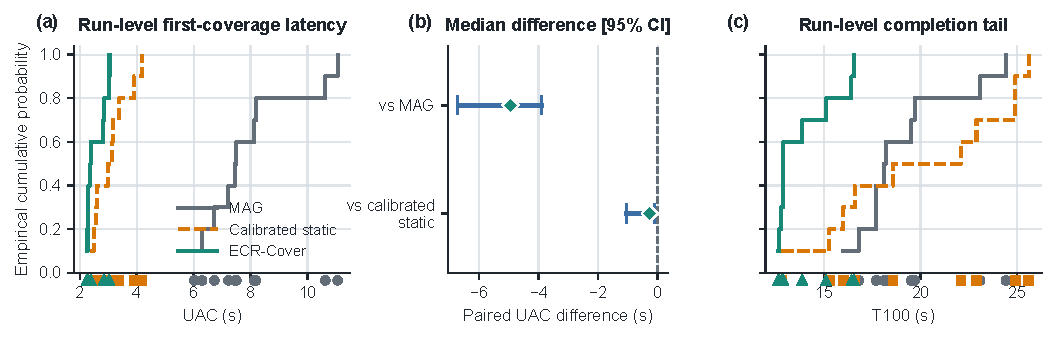
\includegraphics[width=\textwidth]{figure3_nominal.pdf}
\caption{Nominal hardware results, with ten block-level runs per method. (a) Empirical UAC distributions; symbols below the axis are individual runs. (b) Frozen paired median UAC differences and 95\% bootstrap confidence intervals for ECR-Cover relative to MAG and calibrated static planning. (c) Empirical T100 distributions. The forest panel uses the preregistered intervals and does not recompute them.}\label{fig:nominal}
\end{figure*}

\subsection{Temporary Interruption and Repair Ablation}

In the interrupted system-level comparison, median UAC was 3.907~s for ECR-Cover and 5.617~s for calibrated static planning. The paired difference was $-1.134$~s, but its 95\% CI, $[-3.581,1.134]$~s, crossed zero. Median T100 values were 37.866 and 37.302~s. Because the two conditions used different initial routes and differed in online repair, this comparison cannot assign the observed difference specifically to repair. It instead characterizes complete methods under the same pause rule.

The repair switch ablation isolates the mechanism. With the same initial plan and interruption rule, repair-on UAC had a median of 3.549~s and repair-off UAC a median of 5.510~s. The paired median difference was $-1.979$~s with a 95\% CI of $[-2.496,-1.821]$~s. Nine blocks improved and one block was adverse; all ten appear in Figure~\ref{fig:repair}a. The preregistered one-sided exact sign test gave $p=0.010742$. Thus the effect is supported by the direction and interval of run-level paired observations, not by treating cells or control samples as independent replicates.

Repair-on median T95 was 20.206~s, compared with 38.001~s when repair was disabled. Median T100 values were 37.965 and 38.007~s. The paired T100 ratio had a median of 0.998 and a 95\% CI of $[0.954,1.0001]$. Its upper confidence bound was below the preregistered 1.05 noninferiority margin (Figure~\ref{fig:repair}b). The repair-on UAC improvement therefore occurred without evidence of a completion-time penalty beyond that margin.

Each repair-on run committed one effective repair and confirmed at least one reassigned cell before the paused camera recovered. No repair-off run contained such an event. The result supplies the physical witness required to connect Proposition~\ref{prop:repair}'s predicted commit rule to execution: the transferred task was not merely present in a modified queue; it produced a fresh-frame, measured-pose coverage record while the original device was still unavailable.

\begin{figure*}[t]
\centering
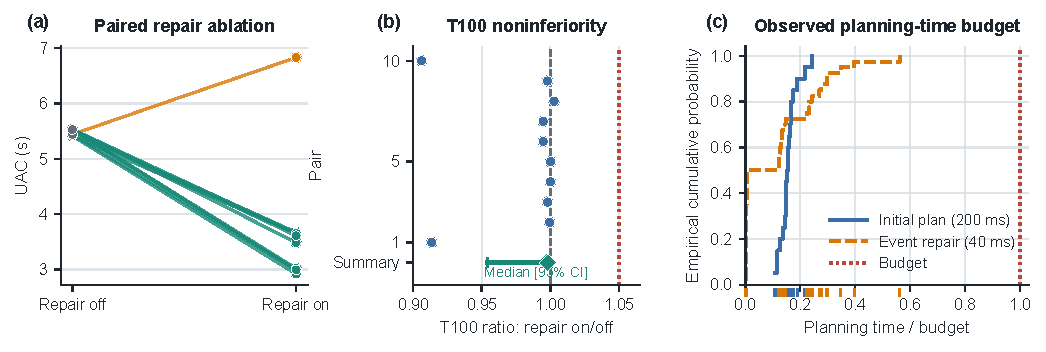
\includegraphics[width=\textwidth]{figure4_repair.pdf}
\caption{Repair ablation and computation budget. (a) UAC for the ten repair-off/on pairs; green lines improve with repair and the orange line is the single adverse pair. (b) The ten T100 ratios and the frozen median 95\% bootstrap interval, with equality at 1.00 and the 5\% noninferiority boundary at 1.05. (c) Empirical planning times normalized by their respective budgets; symbols below the axis retain individual measurements.}\label{fig:repair}
\end{figure*}

\subsection{Execution-Evidence Audit and Computation Budget}

The 70 runs generated 461 coverage-confirmation events. Median absolute azimuth and elevation differences between planned and confirming poses were both $0.5^\circ$; their 95th percentiles were both $0.9^\circ$, and no confirming event exceeded the $1^\circ$ completion gate. Within the frozen projection model, every one of the 461 planning-core cell sets was contained in the field of view projected from the corresponding measured pose, and every logged coverage cell belonged to that measured-pose projection. The planning core and measured-pose footprint contained median counts of 63 and 180 cells, respectively. These checks support consistency between software evidence and the frozen geometry; they do not add an external world-coordinate calibration.

All frames referenced by coverage events passed the logged usability and resolution checks and could be joined to the pose sample, frame identifier, task identifier, and COMPLETE event. One raw unusable-frame status occurred in the repair-ablation archive, but it was not referenced by a coverage event. The ledger therefore reconstructs all reported first-coverage times from qualifying execution events rather than scheduled timestamps.

Across the 20 repair-ablation runs, initial planning time ranged from 21.52 to 48.79~ms, with a median of 30.75~ms, below the 200~ms budget. The 40 pause/recovery planning events ranged from 0.10 to 22.48~ms, with a median of 2.56~ms, below the 40~ms event budget. Figure~\ref{fig:repair}c shows the observations relative to their respective budgets. These measurements establish budget compliance in the frozen Windows/Python platform; they are not a hard real-time schedulability result.

